\documentclass{article}

\usepackage{graphicx}
\usepackage{hyperref}
\hypersetup{%               %           Setup the coloring of the links. 
%                           %           Currently the only necessary one is "colorlinks=true" and "linkcolor=blue".
    colorlinks   = true,    %           Colours links instead of ugly boxes
    urlcolor     = blue,    %           Colour for external hyperlinks
    linkcolor    = blue,    %           Colour of internal links
    citecolor    = blue     %           Colour of citations, could be ``red''
    }
\usepackage[margin=2cm]{geometry}
\title{YouTube Upload Instructions for Lightboard Videos}
\author{Jason Nowell}
\date{}

\begin{document}
\maketitle


This is a guide to uploading and doing very basic video editing of lightboard videos made in the mathematics department lightboard studio.%
\footnote{This guide is accurate as of 2019, however it may require updating due to YouTube studio changes pending litigation unrelated to anything in this guide}%
Note however that YouTube only allows fairly basic video editing; primarily just the ability to crop parts of video. Part one is a very indepth step-by-step guide on how to do everything from logging into the correct YouTube account, to cropping parts of your video and sharing it with students. Part two is a very succinct summary for those that are familiar with the process and only need the very bare minimum of information to proceed.


\tableofcontents

\newpage

\part{In-Depth Tutorial: \\ Step by Step process from Start to Finish}
\label{partOne}
    \section{Logging Into YouTube}
    \label{loggingOn}
        The UF Xronos team has its own dedicated YouTube channel. You can log into this channel using the associated Google Account with the following credentials: (Note: Capitalization is important for the password)
        \begin{description}
            \item[\textbf{Username:}] XronosUF@GMail.com
            \item[\textbf{Password:}] XronosUF2016
        \end{description}
        
        When you initially log into YouTube it may show your channel and, specifically, your "videos". This video list \textit{should be empty}. This is because all our videos are unlisted, which we will cover later in the guide on how to configure the video.
    
    \section{Uploading Video}
        If you have followed the guide on how to use the lightboard, you should already have a video file awaiting upload. For the purposes of this guide we will assume the video is called ``Test Video File". \\
        
        When you log into YouTube using the credentials above, there should be a bar along the top with a camera icon with a $+$ sign inside it, which (when you hover over it) says ``create a video or post" as in Figure \ref{uploadButton}.
        
        \begin{figure}[h]
            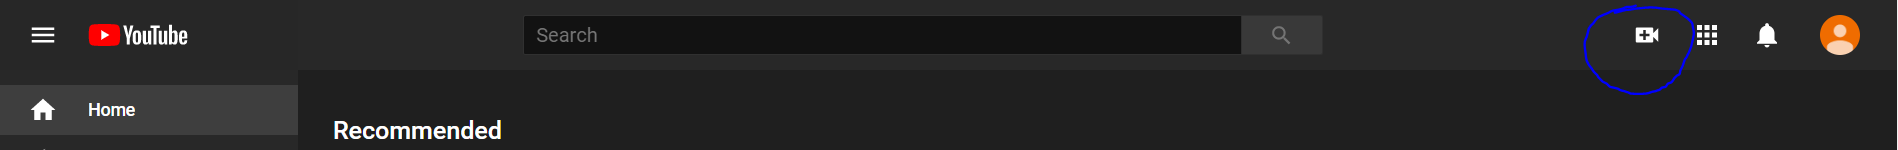
\includegraphics[width=\textwidth]{youTubeUploadButton.png}
            \caption{YouTube upload video button. Alternatively you can click the far right orange button in the picture which will bring up a menu, under which you can click the ``YouTube Studio" and then ``Upload Video" button in the center of the screen.}
            \label{uploadButton}
        \end{figure}
        
        \newpage
        Once you have clicked the ``upload video" button, you should now see something like Figure \ref{selectFile}. Upload your file either by dragging and dropping the video file to the big center arrow, or by clicking the ``select file" button and navigating to your video. 
        
        \begin{figure}[h]
            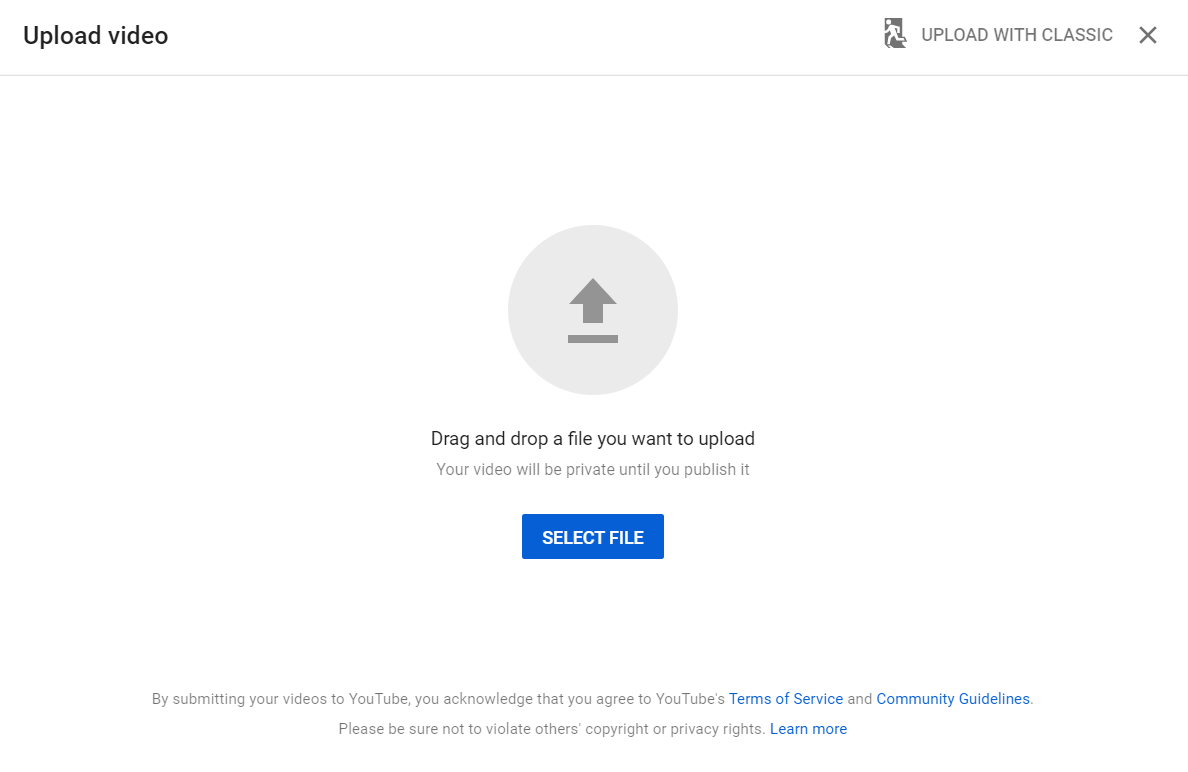
\includegraphics[width=\textwidth]{selectFile.png}
            \caption{This is what you should see when you hit the upload video button. You can either drag your video to the middle of the box, or click the ``Select File" button and navigate to wherever you have saved your file.}
            \label{selectFile}
        \end{figure}    
    \newpage
    \section{Configuring The Video On Upload}
        
        Once you have started the upload process a box will pop up to guide you through the process of configuring the video settings. You can keep most of these settings as they are, but some of them are \textit{very} important to set correctly. 
        
        The first thing you need to set is the title and description of your video. These should reflect what your video is about, as these are the things that your students will see when they first load the video. These are also the settings that are the first to pop up when you are configuring the new uploaded video. Immediately after you drag and drop (or select) the video for upload you should see something like Figure \ref{titleDescription}:
        
        \begin{figure}[h]
            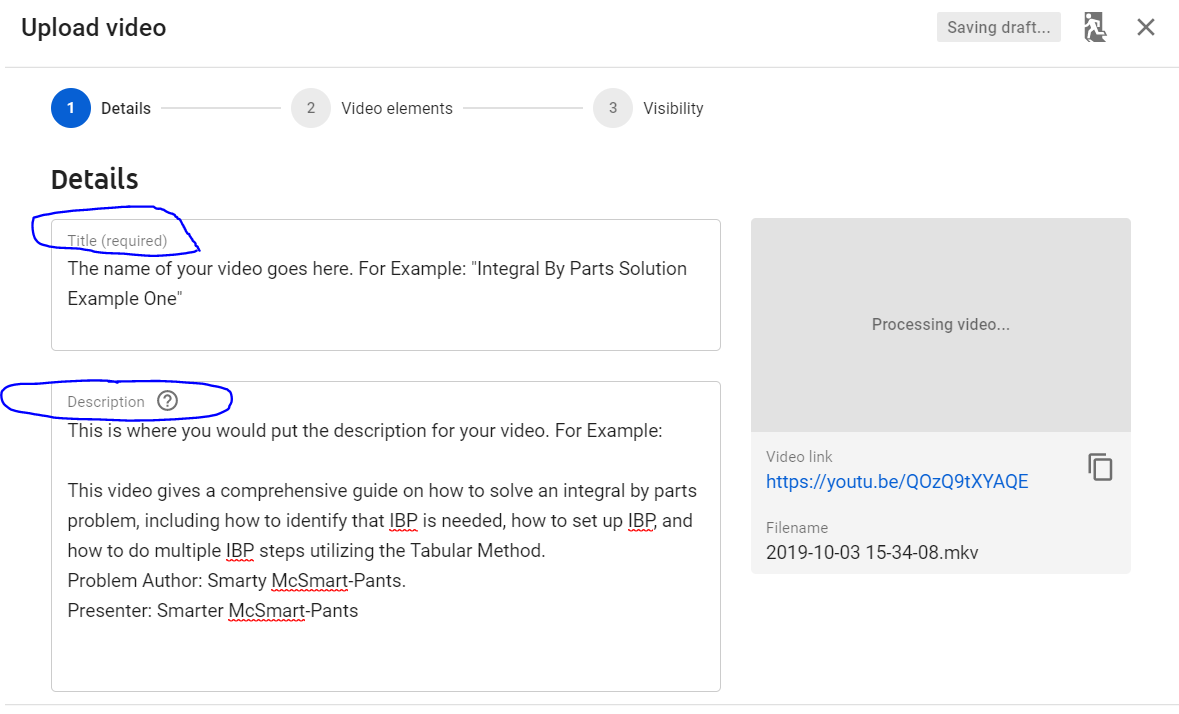
\includegraphics[width=\textwidth]{uploadedVideoTitleDescription.png}
            \caption{This should be the first box to pop up after you start the upload process of your video. You want to fill in the title and description. The fields are indicated in the picture, along with an example for each.}
            \label{titleDescription}
        \end{figure}
        
        \newpage
        
        Once you have set a title and a description, you should scroll down until you see something like Figure \ref{ageMoreOptions}. It is \textit{very important} that you tag your video as ``Not made for kids" (In this context ``kids" is those below the age of 13, and this is a legal distinction, not a comment on if you content can be understood by those under 13.)
    
        \begin{figure}[h]
            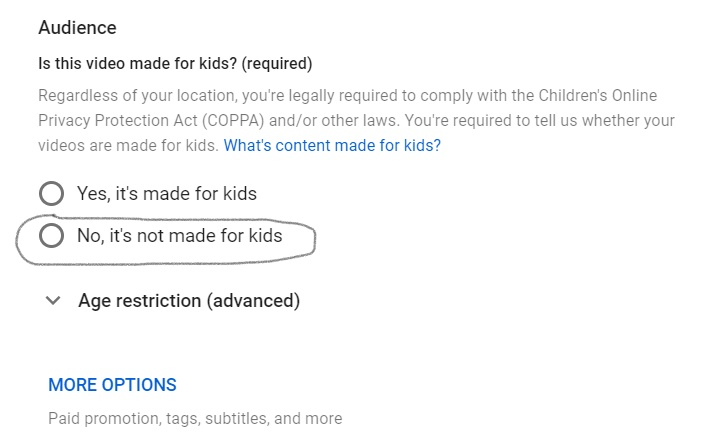
\includegraphics[width=\textwidth]{audienceMoreOptions.png}
            \caption{Make sure to indicate your video is not made for kids. This is for those that are specifically aiming their video content to be targeted toward those under the age of 13, and comes will all kinds of restrictions, technological challenges, and difficulties that will almost certainly make the video inaccessible to a significant number of students.}
            \label{ageMoreOptions}
        \end{figure}    
        
        \newpage
        As can be seen in Figure \ref{ageMoreOptions}, there may be a ``More Options" button, or (depending on changes) you may simply be able to continue scrolling down until you see a sections on tags. It is strongly recommended you include relevant tags for your content here in order to help students find and understand the scope of the intended video. Take a look at Figure \ref{tagSection} for an example of what we might choose as tags for our example.
    
        \begin{figure}[h]
            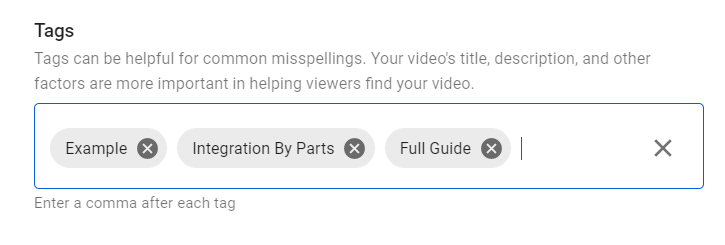
\includegraphics[width=\textwidth]{tagsList.png}
            \caption{Since this is a guide and example problem for IBP, we tagged our video with ``Example", ``Integration By Parts", and ``Full Guide".}
            \label{tagSection}
        \end{figure}
        
        
        \newpage
        Finally, to ``Publish" your video you will want to go to the last tab ``Visibility" and select the ``Unlisted" option, as you can see in Figure \ref{publishVisibility}. Note that, although you are publishing the video nobody will have access to it without your direct link, so you can publish it before you have edited the video (and in fact, you need to). So if you need to edit the video, don't worry, you will do that after this step. 
    
        \begin{figure}[h]
            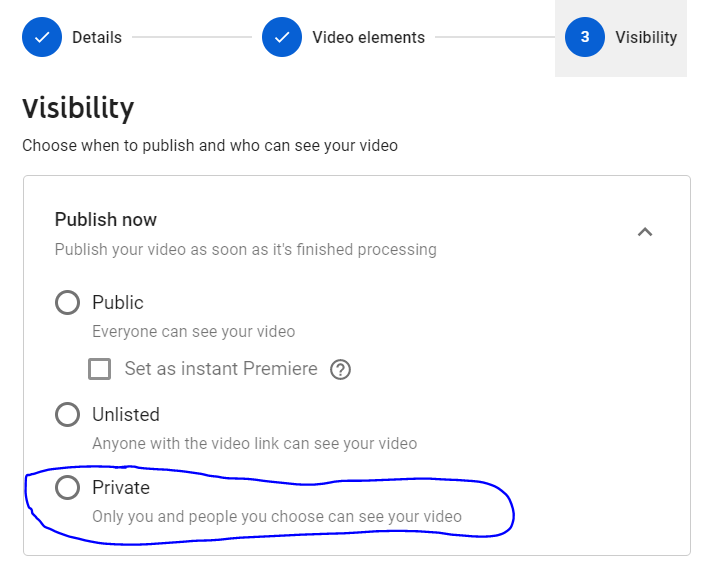
\includegraphics[width=\textwidth]{publishVisibility.png}
            \caption{Make sure to select the ``Unlisted" option. You may have to hit the arrow next to the ``Publish Now" option to be able to see the unlisted option first. We don't need to do anything in the ``Video Elements" section, so you can skip this section of the upload configuration section.}
            \label{publishVisibility}
        \end{figure}
    
    \newpage
    
    \section{How To Crop Video}
        
        Once you have finished uploading a video you should be brought to the YouTube Studio Video page. This page lists all videos that have been uploaded to the YouTube channel (included everyone elses videos!) You should see something like Figure \ref{studioHome}
        
        \begin{figure}[h]
            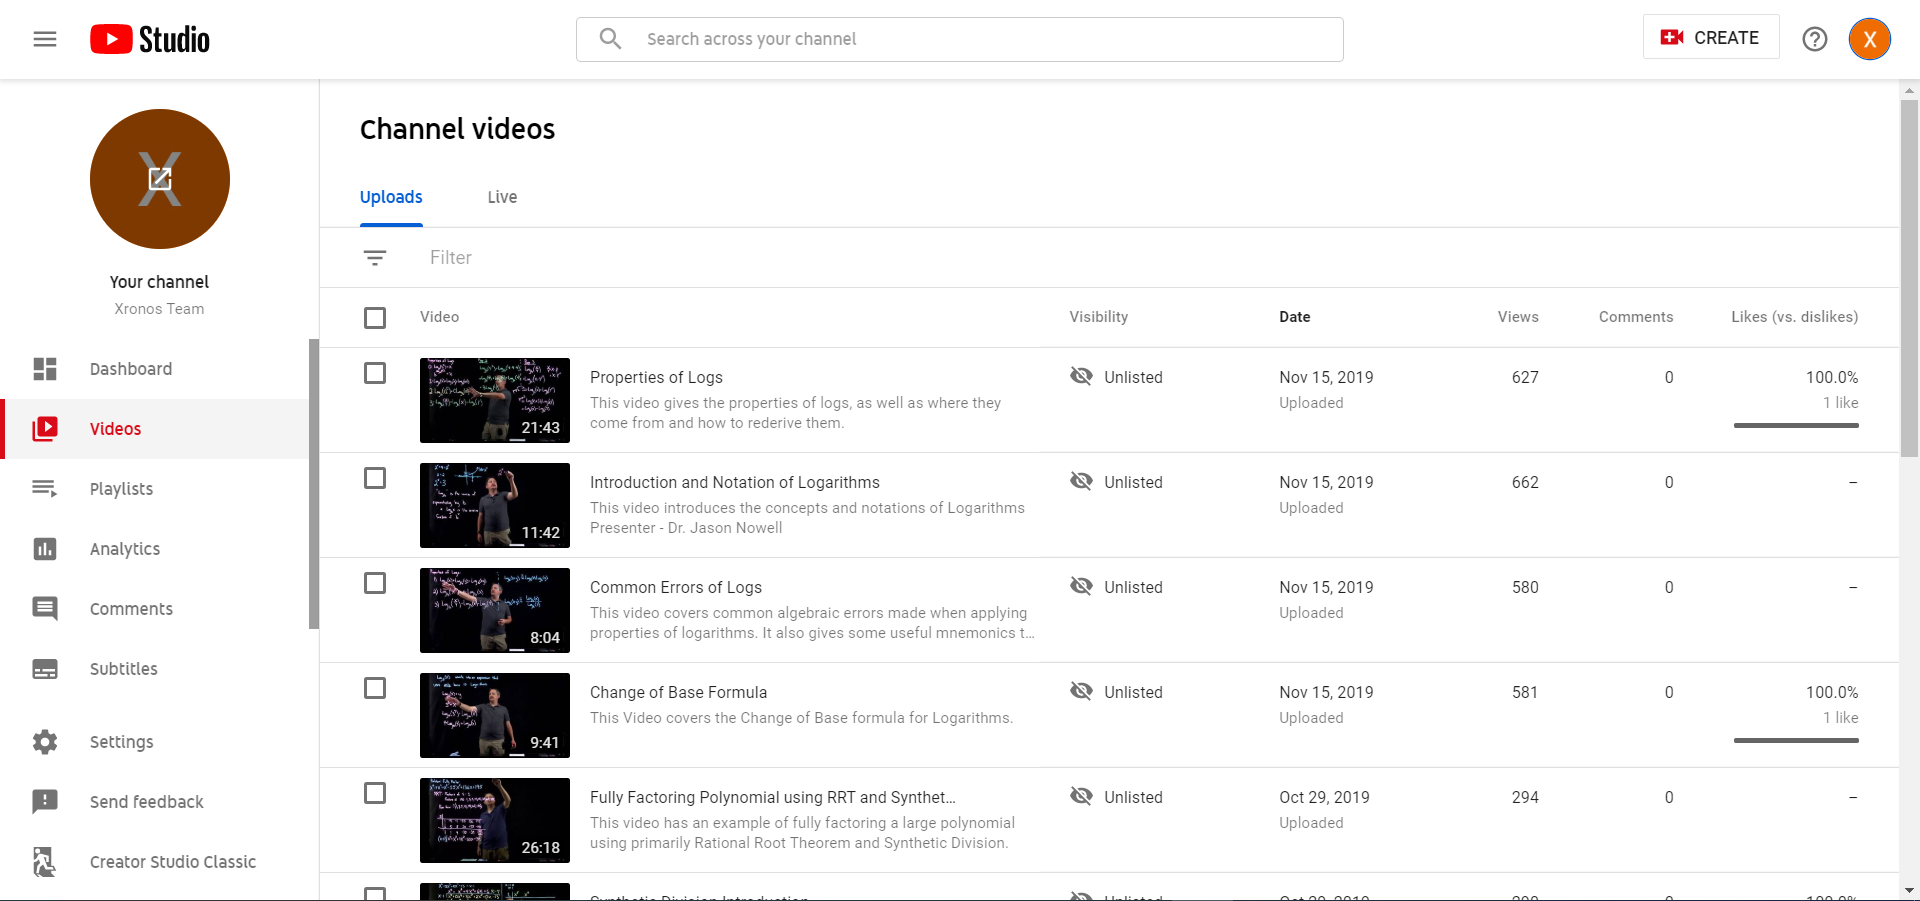
\includegraphics[width=\textwidth]{studioHomePage.png}
            \caption{This is the YouTube Studio Video Homepage. If you don't load to this directly, you can access it video the top right orange button and going to YouTube Studio page, then clicking ``Videos" on the far left as shown in this figure.}
            \label{studioHome}
        \end{figure}
        
        You want to click on your own video in order to load that video's settings and to be able to start the editing process.
        
        \newpage
        
        Once you have clicked on your video the video settings summary page will load. It should look something like Figure \ref{videoDetails}. The areas circled in blue should already be set from earlier in our tutorial, but you should double check and make sure that they are configured correctly. In particular, make sure that it is set to ``Not intended for Kids" and that the visibility is ``Unlisted". The red section is a new optional setting that lets you choose what students see when they see the video before hitting play (for example, what they see when the video is embedded in a Xronos page, before they start playing it). Finally the green circled content is the link directly to this video. You will need this link in order to embed and/or give the link directly to your students. Since the video is unlisted, there is no other way for anyone to access the video.
        
        \begin{figure}[h]
            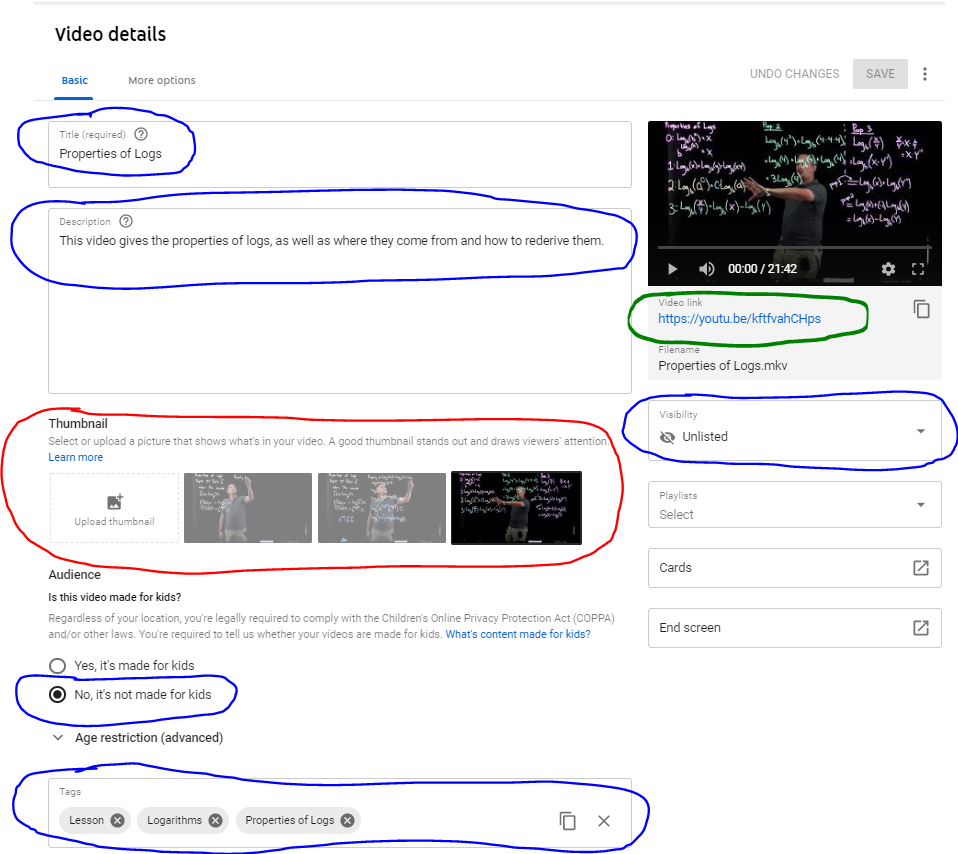
\includegraphics[width=\textwidth]{videoDetails.png}
            \caption{Verify that all the settings are as intended before moving on to edit your video.}
            \label{videoDetails}
        \end{figure}
        
        \newpage
        
        Now that you have verified all the settings you need for your video, along the far left hand side should be a vertical navigation bar; one option is ``Editor''. You want to click this to bring up the editing page for your particular video, which should look something like Figure \ref{editingPage}. The caption explains the various parts of interest on this page, but in particular you will want to press the ``Trim'' button to start the process of cropping your video to get rid of the beginning and tail sections of the video that you don't want (when you are walking around the screen after hitting start recording at the computer, or on your way to hit end recording at the computer).
    
        \begin{figure}[h]
            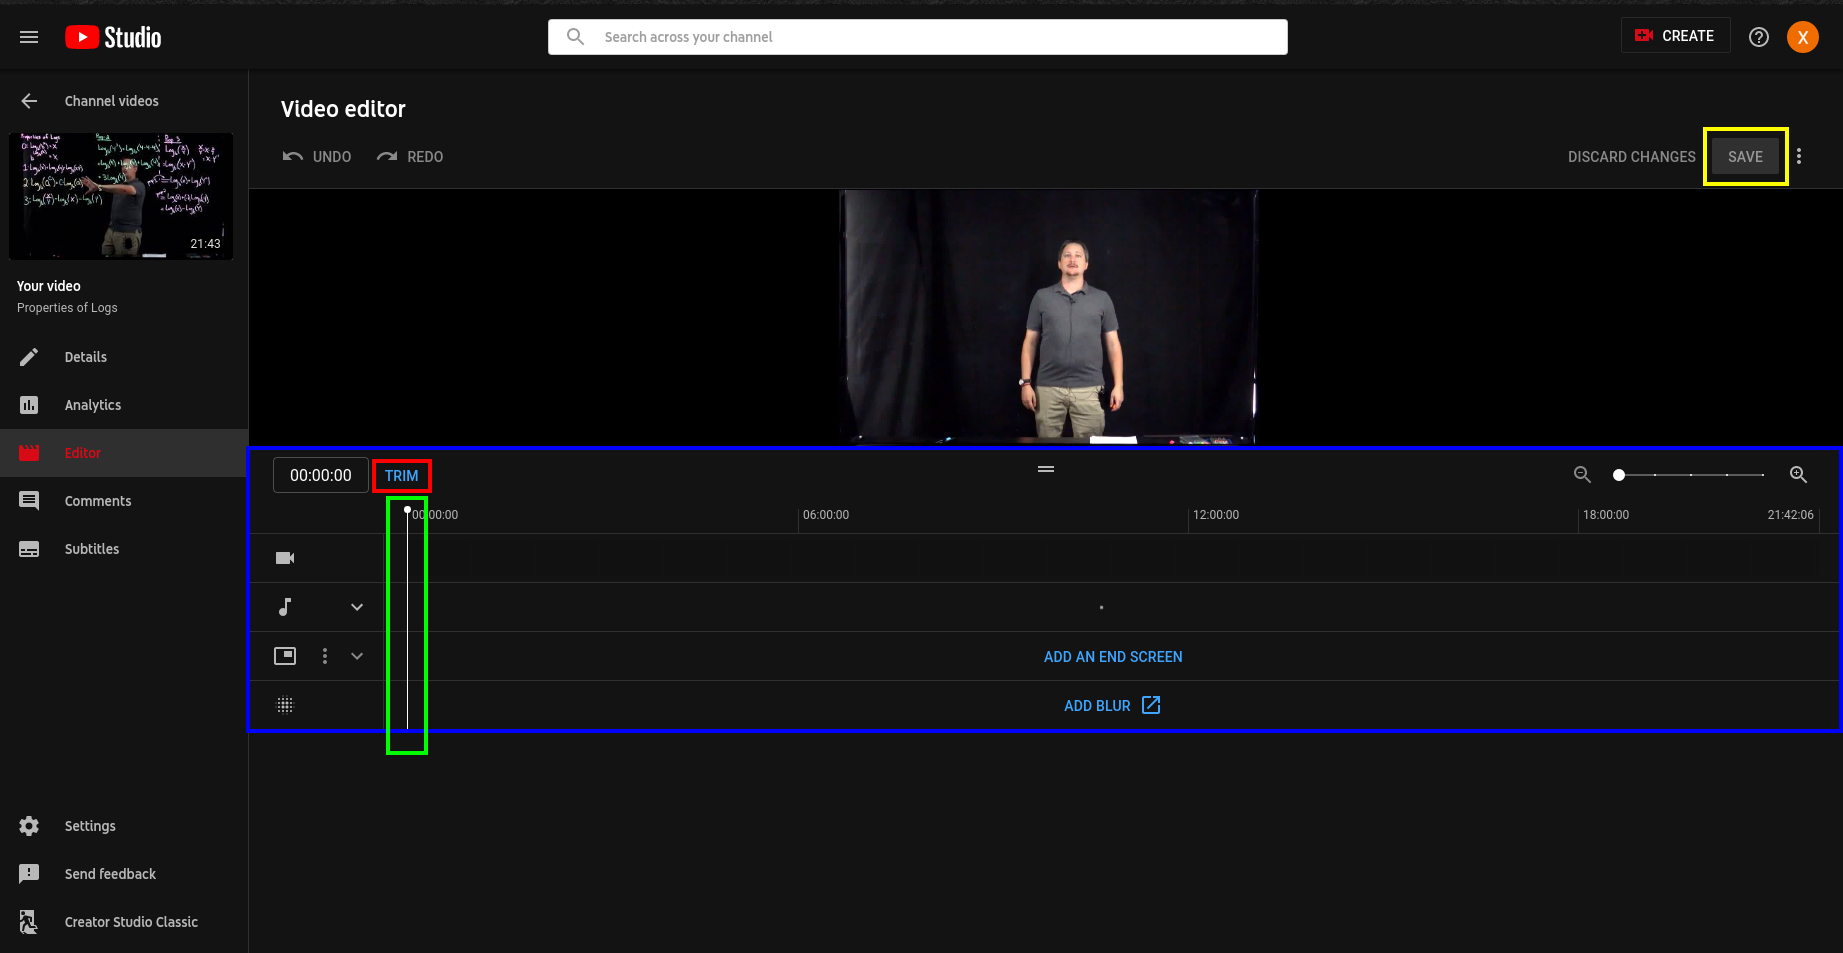
\includegraphics[width=\textwidth]{editingPage.png}
            \caption{There are three things in particular that you will want to use while editing. The blue box is the general area you will be working in; this will show your crops and edits. The green box around the vertical bar shows where your current placement in the video is. Finally the red box is the ``Trim'' button which is what you will want to press to bring up the crop options.}
            \label{editingPage}
        \end{figure}
        
        \newpage
        
        Once you hit the ``Trim'' button you should see something like Figure \ref{trimPage} on your screen. Notice at the button that you should see the blue bar with ``Split'' as an option. If you click this button it will start a crop at the current timestamp, where your vertical white line is on the video progression bar (green box). Once you split the video you can then drag the progression bar to the right or left to cut out that segment of video. You will see what is cut out as it will appear grayed out, as in Figure \ref{postTrim}
    
        \begin{figure}[h]
            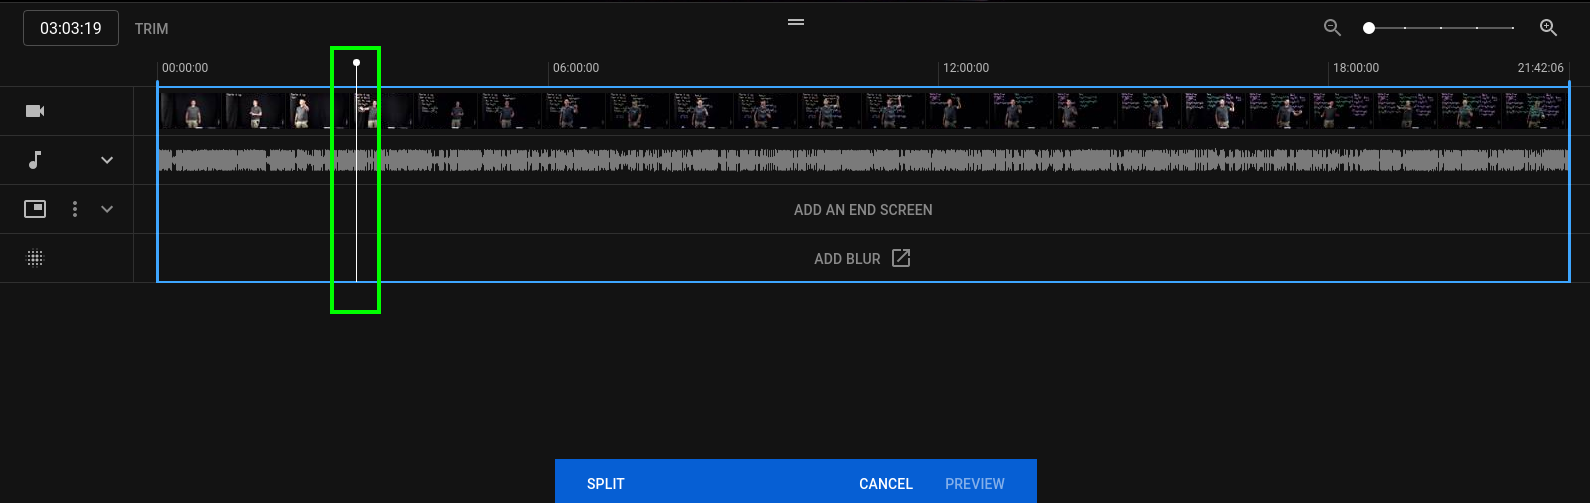
\includegraphics[width=\textwidth]{trimPage.png}
            \caption{This is what it looks like when you have pressed the ``Trim'' button. Notice the ``Split'' button at the bottom in the blue bar; pressing this will cut the video at the current time mark (indicated by the progress line in the green box) and allow you to trim to the right or left of the video.}
            \label{trimPage}
        \end{figure}
        
        \begin{figure}[h]
            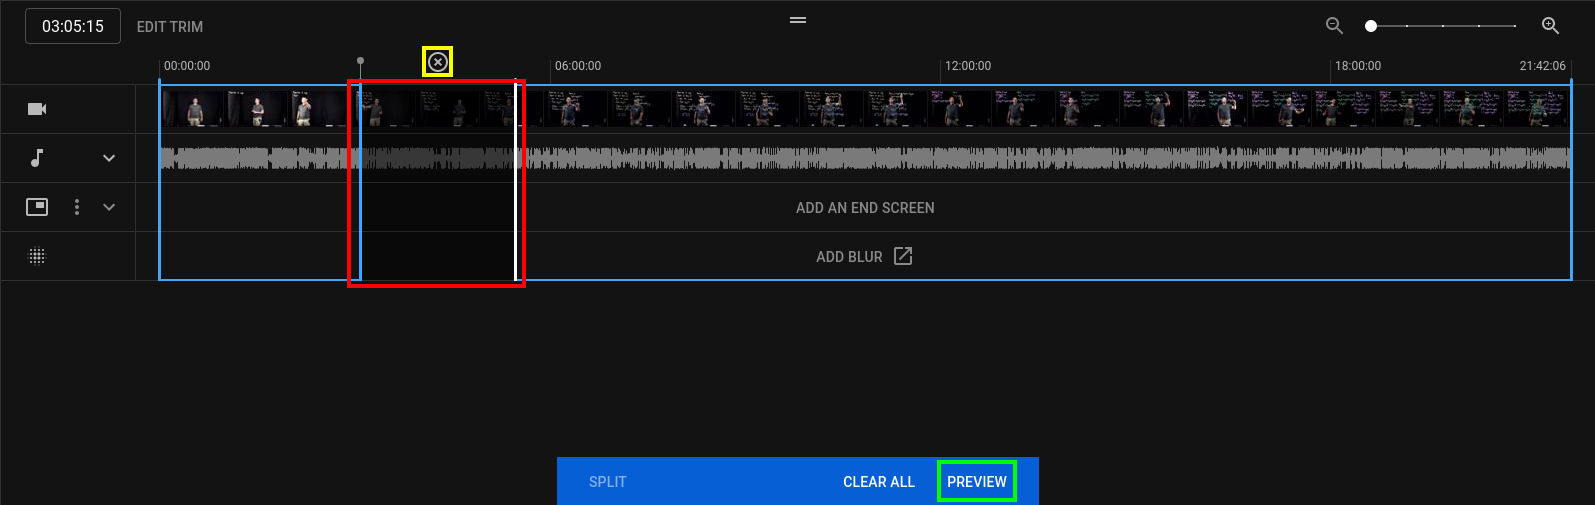
\includegraphics[width=\textwidth]{postTrim.png}
            \caption{Notice that we have trimmed some of the video out here, which is indicated by the grayed out section of the video progression bar (Indicated by the red box). Moreover if you wish to remove this trimming you can do so by clicking the $\textcircled{x}$ button above the trimmed section (indicated by the yellow box.)}
            \label{postTrim}
        \end{figure}
        
        Keep in mind that you only want to use the split button once per trimmed section. You don't want to try and split on either side of the trimmed section and then link them as the YouTube editor gets pretty confused by this. This means you should usually only need to activate the split section twice; once for the start and once for the end. 
        
        As a suggestion, it is usually easiest to navigate to the exact moment you want the video to start or stop, hit the split button there, and then drag the progress bar to the start (or end respectively) to trim off the beginning or end section of the video, rather than hitting the split button early and trying to drag it to the right location.
        
        Finally, note that the video section in the middle of the screen is an active representation of the video, as it exists with current edits. This means that you can mouse over the video in the top-middle of the screen and hit play, and it will play, obeying all the trimmed content that you have removed, before you ``save changes''. This means you can watch your video with all the cropping done (including any mid-video cropping you may want to do) and make sure that everything presents nicely before you commit to the saved results.
        
        Once you have finished making all the edits you want to make for your video, you want to hit the ``preview'' button in the bottom blue box (green box in Figure \ref{postTrim}). This will allow you to hit the ``Save'' button in the top right above the video preview (Yellow box in Figure \ref{editingPage}) to save your video. YouTube will take time to perform the edits and post the new video, at which point you can provide the link to your students (or embed it into Xronos) and your students will have access to to your new Lightboard Video!
        
        
        \newpage
\part{Quick Guide: \\ For Those Familiar with Most or All of the Process}

    This is intended for those that are tech savvy, or have already done this but need a quick reference/refresher on what needs to be done. If you don't know anything about posting a video on YouTube, you should read the more comprehensive guide in \hyperref[partOne]{Part One}. For Login info to access the Xronos YouTube video channel, see the section on \hyperref[loggingOn]{Logging On to YouTube}.
    
    \section{Settings}
    
        The settings you want to set all included in the following picture. Note that it is \textit{very} important to set the ``Content Not Intended for Children'' setting to ensure that embedding and access works.
    
        \begin{figure}[h]
            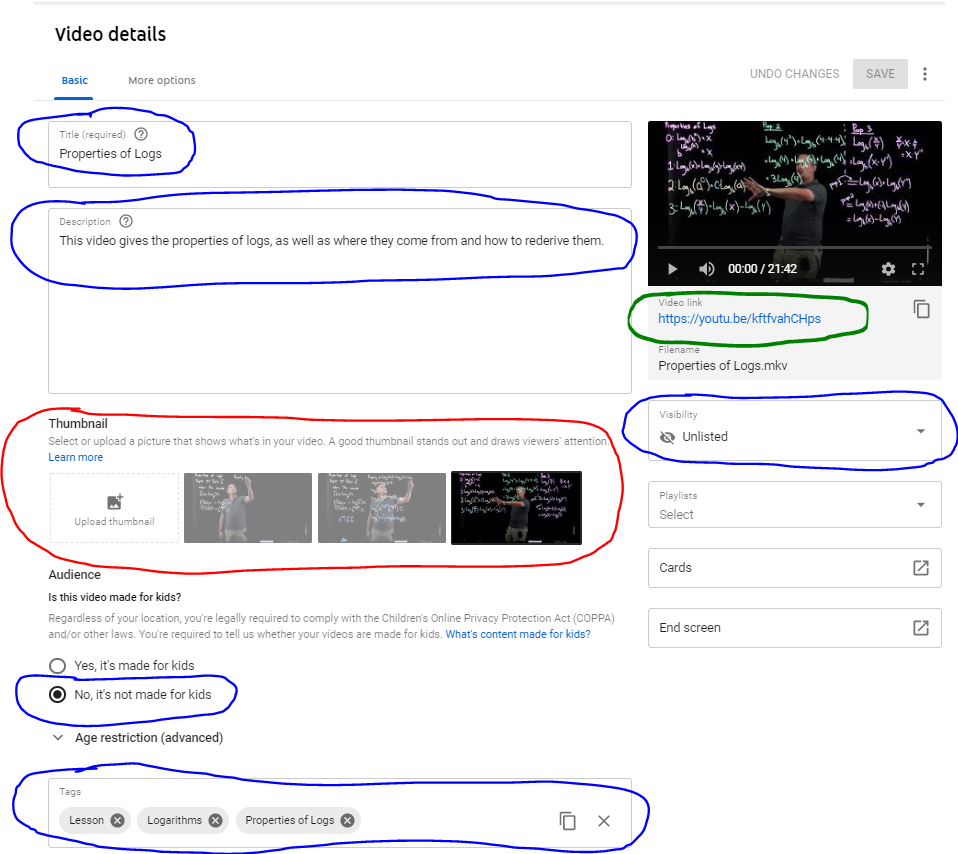
\includegraphics[width=0.7\textwidth]{videoDetails.png}
            \caption{Verify that all the settings are as intended before moving on to edit your video. The ``No it's not made for kids'' option is very important, and the title is necessary. Also make sure to mark visibility as ``unlisted''. The rest is optional but highly suggested. The embedding/sharing link is circled in green.}
        \end{figure}
    
    \newpage
    
    \section{Editing}
        
        You will want to use YouTube Studio to trim the video, in particular the beginning and the ending of the video to remove unwanted content. Do this by accessing the ``Editor'' option on the far left side of the screen once you are in your video's settings section. Once there, hit the Trim button to open up the cropping tool (Red Box in Figure \ref{editingPage}). Crop as desired, by navigating to where you want to start (or end) your crop and pressing the ``Split'' button that appears at the bottom of the page, then dragging the video pregession slider in whichever direction you want to crop until the desired amount of video is removed.
        
        Once you have performed all the cropping you need, hit the Preview button in the bottom panel, and then the save button in the top right (yellow box in Figure \ref{editingPage}). This will save the edited video and post it on YouTube for you once YouTube has finished the remux of the video.



\end{document}